\newpage
\subsection{Mapping water quality with drones: Test case in Texel} \label{similarprojects/multispectral}

As published in the IADC Dredging journal of December 2019, \cite{terraetaqua} a pilot test case at the Prins Hendrik Zanddijk project in Texel, The Netherlands, was organised to demonstrate drone technology for turbidity monitoring. An octocopter drone platform, Altura Zenith ATX8, was used with a multispectral camera, MicaSense RedEdge M, underneath.

The drone data was processed into turbidity maps. Water samples, collected simultaneously with drone flights were used for the validation of the sensor data.\\

The team noted that working with optical sensors add additional challenges. Water surfaces act as a mirror, and when sun light is reflected at the water surface, it is captured by the sensor. This results in a sun glints from which it is hard to obtain information on the water itself. Additionally, varying illumination conditions make it harder to quantify results.

\begin{figure}[h]
\centering
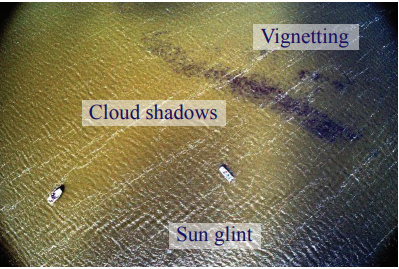
\includegraphics[scale=1]{similarprojects/31_uncorrected.png}
\caption{Uncorrected image with sun glint \cite{terraetaqua}}
\end{figure}

As shown in the publication, some of these problems can be mitigated by slightly tilting the camera and creating flight plans which look away from the sun. The remaining artifacts can be filtered out by an image processing chain.

The results of the pilot test case was positive, with the turbidity values obtained from the drone imagery being within range of manual measurements, though the validation dataset available is pretty small.

The authors stated that in the future, a semi-autonomous data collection architecture can be made where a drone can be triggered by other sensors when these sensors detect an anomaly, performing a defined flight mission.

\subsection{Similarity}
While this project may make use of optical sensors for the assessment of water quality, both projects definitely do have aspirations of being autonomously monitored. The test case opted for a non-waterproof octocopter as the UAV doesn't have to land in the water.